% Created by tikzDevice version 0.12 on 2019-06-13 14:17:53
% !TEX encoding = UTF-8 Unicode
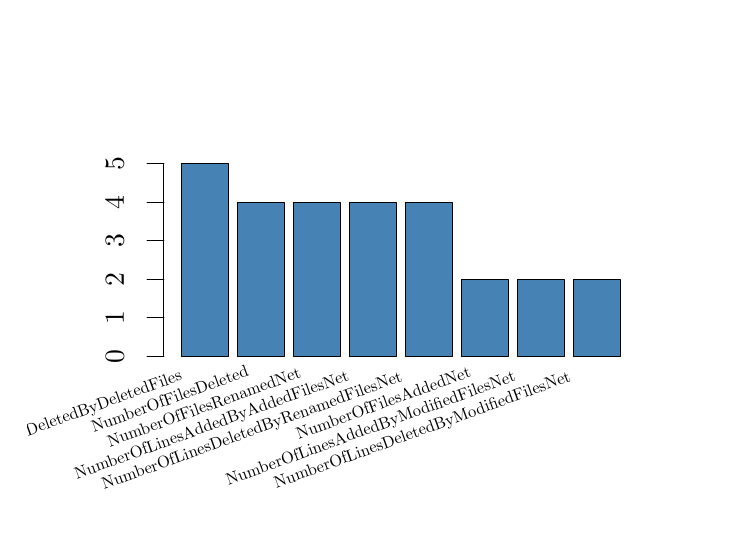
\begin{tikzpicture}[x=1pt,y=1pt]
\definecolor{fillColor}{RGB}{255,255,255}
\path[use as bounding box,fill=fillColor,fill opacity=0.00] (0,0) rectangle (245.72,180.67);
\begin{scope}
\path[clip] (  0.00,  0.00) rectangle (245.72,180.67);
\definecolor{drawColor}{RGB}{0,0,0}
\definecolor{fillColor}{RGB}{70,130,180}

\path[draw=drawColor,line width= 0.4pt,line join=round,line cap=round,fill=fillColor] ( 55.55, 61.90) rectangle ( 72.42,131.47);

\path[draw=drawColor,line width= 0.4pt,line join=round,line cap=round,fill=fillColor] ( 75.80, 61.90) rectangle ( 92.67,117.56);

\path[draw=drawColor,line width= 0.4pt,line join=round,line cap=round,fill=fillColor] ( 96.05, 61.90) rectangle (112.92,117.56);

\path[draw=drawColor,line width= 0.4pt,line join=round,line cap=round,fill=fillColor] (116.30, 61.90) rectangle (133.17,117.56);

\path[draw=drawColor,line width= 0.4pt,line join=round,line cap=round,fill=fillColor] (136.55, 61.90) rectangle (153.42,117.56);

\path[draw=drawColor,line width= 0.4pt,line join=round,line cap=round,fill=fillColor] (156.80, 61.90) rectangle (173.67, 89.73);

\path[draw=drawColor,line width= 0.4pt,line join=round,line cap=round,fill=fillColor] (177.05, 61.90) rectangle (193.92, 89.73);

\path[draw=drawColor,line width= 0.4pt,line join=round,line cap=round,fill=fillColor] (197.30, 61.90) rectangle (214.17, 89.73);
\end{scope}
\begin{scope}
\path[clip] (  0.00,  0.00) rectangle (245.72,180.67);
\definecolor{drawColor}{RGB}{0,0,0}

\path[draw=drawColor,line width= 0.4pt,line join=round,line cap=round] ( 49.20, 61.90) -- ( 49.20,131.47);

\path[draw=drawColor,line width= 0.4pt,line join=round,line cap=round] ( 49.20, 61.90) -- ( 43.20, 61.90);

\path[draw=drawColor,line width= 0.4pt,line join=round,line cap=round] ( 49.20, 75.81) -- ( 43.20, 75.81);

\path[draw=drawColor,line width= 0.4pt,line join=round,line cap=round] ( 49.20, 89.73) -- ( 43.20, 89.73);

\path[draw=drawColor,line width= 0.4pt,line join=round,line cap=round] ( 49.20,103.64) -- ( 43.20,103.64);

\path[draw=drawColor,line width= 0.4pt,line join=round,line cap=round] ( 49.20,117.56) -- ( 43.20,117.56);

\path[draw=drawColor,line width= 0.4pt,line join=round,line cap=round] ( 49.20,131.47) -- ( 43.20,131.47);

\node[text=drawColor,rotate= 90.00,anchor=base,inner sep=0pt, outer sep=0pt, scale=  1.00] at ( 34.80, 61.90) {0};

\node[text=drawColor,rotate= 90.00,anchor=base,inner sep=0pt, outer sep=0pt, scale=  1.00] at ( 34.80, 75.81) {1};

\node[text=drawColor,rotate= 90.00,anchor=base,inner sep=0pt, outer sep=0pt, scale=  1.00] at ( 34.80, 89.73) {2};

\node[text=drawColor,rotate= 90.00,anchor=base,inner sep=0pt, outer sep=0pt, scale=  1.00] at ( 34.80,103.64) {3};

\node[text=drawColor,rotate= 90.00,anchor=base,inner sep=0pt, outer sep=0pt, scale=  1.00] at ( 34.80,117.56) {4};

\node[text=drawColor,rotate= 90.00,anchor=base,inner sep=0pt, outer sep=0pt, scale=  1.00] at ( 34.80,131.47) {5};
\end{scope}
\begin{scope}
\path[clip] (  0.00,  0.00) rectangle (245.72,180.67);
\definecolor{drawColor}{RGB}{0,0,0}

\node[text=drawColor,rotate= 20.00,anchor=base east,inner sep=0pt, outer sep=0pt, scale=  0.60] at ( 56.05, 53.47) {NumberOfLinesDeletedByDeletedFiles};

\node[text=drawColor,rotate= 20.00,anchor=base east,inner sep=0pt, outer sep=0pt, scale=  0.60] at ( 80.16, 54.88) {NumberOfFilesDeleted};

\node[text=drawColor,rotate= 20.00,anchor=base east,inner sep=0pt, outer sep=0pt, scale=  0.60] at ( 99.10, 54.40) {NumberOfFilesRenamedNet};

\node[text=drawColor,rotate= 20.00,anchor=base east,inner sep=0pt, outer sep=0pt, scale=  0.60] at (116.46, 53.35) {NumberOfLinesAddedByAddedFilesNet};

\node[text=drawColor,rotate= 20.00,anchor=base east,inner sep=0pt, outer sep=0pt, scale=  0.60] at (135.73, 53.00) {NumberOfLinesDeletedByRenamedFilesNet};

\node[text=drawColor,rotate= 20.00,anchor=base east,inner sep=0pt, outer sep=0pt, scale=  0.60] at (160.54, 54.66) {NumberOfFilesAddedNet};

\node[text=drawColor,rotate= 20.00,anchor=base east,inner sep=0pt, outer sep=0pt, scale=  0.60] at (176.64, 53.14) {NumberOfLinesAddedByModifiedFilesNet};

\node[text=drawColor,rotate= 20.00,anchor=base east,inner sep=0pt, outer sep=0pt, scale=  0.60] at (196.62, 53.04) {NumberOfLinesDeletedByModifiedFilesNet};
\end{scope}
\end{tikzpicture}
